% Gabarit pandoc des corrigés publiés (brut et guidé). Contenu sans marque ni nom de site.
% Compilation : lualatex (latexmk -lualatex).
% Le Markdown reste la source unique : ne pas éditer ce fichier .tex à la main.
\documentclass[11pt,a4paper]{article}

% --- Moteur, polices (Latin Modern) et langue ---------------------------------
\usepackage{iftex}
\ifLuaTeX\else\errmessage{Ce document se compile avec lualatex}\fi
\usepackage{amsmath,amssymb,mathtools}
\usepackage{fontspec}
% mathrm=sym : \mathrm prend ses glyphes dans la police mathématique (ℓ, μ, Ω), comme KaTeX.
\usepackage[math-style=TeX,bold-style=TeX,mathrm=sym]{unicode-math}
% Repli pour les glyphes absents de Latin Modern (indices et exposants Unicode,
% flèches, filets des schémas en texte, symboles) : DejaVu, puis Latin Modern Math
% (ℓ, lettres mathématiques Unicode des légendes).
\directlua{
  luaotfload.add_fallback("repliTexte", {"DejaVuSerif:mode=harf;", "DejaVuSans:mode=harf;", "file:latinmodern-math.otf:mode=harf;"})
  luaotfload.add_fallback("repliMono", {"DejaVuSansMono:mode=harf;", "DejaVuSans:mode=harf;", "file:latinmodern-math.otf:mode=harf;"})
}
\setmainfont{Latin Modern Roman}[RawFeature={fallback=repliTexte}]
\setsansfont{Latin Modern Sans}[RawFeature={fallback=repliTexte}]
\setmonofont{Latin Modern Mono}[RawFeature={fallback=repliMono}]
\setmathfont{Latin Modern Math}
\usepackage[french]{babel}
\frenchsetup{SmallCapsFigTabCaptions=false}

% --- Mise en page --------------------------------------------------------------
\usepackage[a4paper,margin=2.2cm,headheight=14pt,footskip=1.2cm]{geometry}
\usepackage{microtype}
\setlength{\emergencystretch}{4em}
\tolerance=1500
\setlength{\parindent}{0pt}
\setlength{\parskip}{0.55\baselineskip plus 2pt minus 1pt}
\usepackage{xcolor}
% Gris nommés : babel-french rend « ! » actif dans le document.
\definecolor{gris2}{gray}{0.98}
\definecolor{gris3}{gray}{0.97}
\definecolor{gris5}{gray}{0.95}
\definecolor{gris35}{gray}{0.65}
\definecolor{gris40}{gray}{0.60}
\definecolor{gris45}{gray}{0.55}
\definecolor{gris50}{gray}{0.50}
\definecolor{gris55}{gray}{0.45}
\definecolor{gris60}{gray}{0.40}
\definecolor{gris65}{gray}{0.35}
\definecolor{gris70}{gray}{0.30}
\definecolor{gris80}{gray}{0.20}
\definecolor{gris85}{gray}{0.15}
\usepackage{graphicx}
\usepackage{float}
\usepackage{caption}
\captionsetup{font=small,labelformat=empty,justification=centering}
\usepackage{booktabs,longtable,array,multirow,calc}
\usepackage{siunitx}
\sisetup{locale=FR}
\usepackage[version=4]{mhchem}
\usepackage{listings}
\usepackage{fancyhdr}
\usepackage{lastpage}
\usepackage[most]{tcolorbox}
\usepackage{enumitem}
\setlist{nosep,leftmargin=*,topsep=2pt}
\usepackage[hidelinks,unicode]{hyperref}
\usepackage{bookmark}
\hypersetup{pdftitle={ATS — Sciences industrielles 2026},pdfauthor={Rédigé par IA},pdfcreator={LaTeX},pdfsubject={Corrigé brut}}
\usepackage{xurl}

% --- Pandoc : listes, tableaux, figures ----------------------------------------
\providecommand{\passthrough}[1]{#1}
\providecommand{\tightlist}{\setlength{\itemsep}{0pt}\setlength{\parskip}{0pt}}

\makeatletter
\def\maxwidth{\ifdim\Gin@nat@width>\linewidth\linewidth\else\Gin@nat@width\fi}
\def\maxheight{\ifdim\Gin@nat@height>0.55\textheight 0.55\textheight\else\Gin@nat@height\fi}
\makeatother
\setkeys{Gin}{width=\maxwidth,height=\maxheight,keepaspectratio}
\setcounter{secnumdepth}{-\maxdimen}
\providecommand{\pandocbounded}[1]{#1}
\usepackage{longtable,booktabs,array}

% --- Code (listings) -----------------------------------------------------------
\lstset{
  basicstyle=\ttfamily\small,
  columns=fullflexible,
  keepspaces=true,
  breaklines=true,
  breakatwhitespace=false,
  postbreak=\mbox{\textcolor{gris50}{$\hookrightarrow$}\space},
  frame=single,
  rulecolor=\color{gris35},
  framesep=4pt,
  xleftmargin=5pt,xrightmargin=5pt,
  backgroundcolor=\color{gris3},
  keywordstyle=\bfseries,
  commentstyle=\color{gris65},
  stringstyle=\color{gris80},
  showstringspaces=false,
  tabsize=4,
  extendedchars=true,
  aboveskip=6pt,belowskip=6pt,
}

% --- Macros des corrigés (KaTeX ↔ LaTeX) ---------------------------------------
% Les corrigés sont écrits pour KaTeX : on définit ici ce que KaTeX connaît et
% que LaTeX n'a pas, sans jamais retoucher le Markdown.
\providecommand{\R}{\mathbb{R}}
\providecommand{\N}{\mathbb{N}}
\providecommand{\Z}{\mathbb{Z}}
\providecommand{\Q}{\mathbb{Q}}
\providecommand{\C}{\mathbb{C}}
\providecommand{\dd}{\mathrm{d}}
\providecommand{\llbracket}{\lBrack}
\providecommand{\rrbracket}{\rBrack}
\providecommand{\lBrace}{\lbrace}
\providecommand{\rBrace}{\rbrace}
\providecommand{\Box}{\square}
\providecommand{\Diamond}{\lozenge}
\providecommand{\varnothing}{\emptyset}
\providecommand{\argmax}{\operatorname*{arg\,max}}
\providecommand{\argmin}{\operatorname*{arg\,min}}
\renewcommand{\leq}{\leqslant}
\renewcommand{\geq}{\geqslant}

% Équation hors texte : réduite à la largeur de la ligne si elle déborde.
\newsavebox{\boiteequation}
\newcommand{\equationajustee}[1]{%
  \sbox{\boiteequation}{$\displaystyle #1$}%
  \ifdim\wd\boiteequation>\linewidth
    \[\resizebox{\linewidth}{!}{\usebox{\boiteequation}}\]%
  \else
    \[#1\]%
  \fi}

% --- Encadrés pédagogiques (sobres, lisibles en noir et blanc) -----------------
\tcbset{
  encadre/.style={
    enhanced,breakable,sharp corners,
    colback=white,colframe=gris55,
    boxrule=0.4pt,leftrule=2.2pt,
    left=6pt,right=6pt,top=3pt,bottom=3pt,
    before skip=6pt,after skip=6pt,
    fonttitle=\bfseries\small,coltitle=black,
    attach title to upper,after title={\quad},
    parbox=false,
  }
}
\newtcolorbox{indication}[1]{encadre,colframe=gris45,colback=gris2,title={Indication~#1}}
\newtcolorbox{methode}{encadre,colframe=gris70,title={Méthode}}
\newtcolorbox{piege}{encadre,colframe=gris85,boxrule=0.8pt,leftrule=2.2pt,title={Piège}}
\newtcolorbox{jury}{encadre,colframe=gris60,colback=gris5,title={Jury}}
\newtcolorbox{encadrenote}{encadre,colframe=gris40}

% --- Titres de section ---------------------------------------------------------
\usepackage{titlesec}
\titleformat{\section}{\Large\bfseries}{}{0pt}{}
\titleformat{\subsection}{\large\bfseries}{}{0pt}{}
\titleformat{\subsubsection}{\normalsize\bfseries}{}{0pt}{}
\titlespacing*{\section}{0pt}{14pt plus 4pt minus 2pt}{6pt}
\titlespacing*{\subsection}{0pt}{10pt plus 3pt minus 2pt}{4pt}
\titlespacing*{\subsubsection}{0pt}{8pt plus 2pt minus 2pt}{2pt}

% --- En-tête et pied de page ---------------------------------------------------
\pagestyle{fancy}
\fancyhf{}
\fancyhead[L]{\small\textsc{Corrigé brut} · ATS ATS}
\fancyhead[R]{\small Sciences industrielles 2026}
\fancyfoot[L]{\footnotesize Corrigé rédigé par IA, non officiel}
\fancyfoot[R]{\footnotesize \thepage\,/\,\pageref*{LastPage}}
\renewcommand{\headrulewidth}{0.4pt}
\renewcommand{\footrulewidth}{0pt}
\fancypagestyle{plain}{\fancyhf{}\fancyfoot[R]{\footnotesize \thepage\,/\,\pageref*{LastPage}}\fancyfoot[L]{\footnotesize Corrigé rédigé par IA, non officiel}\renewcommand{\headrulewidth}{0pt}}

\begin{document}
\thispagestyle{plain}
\begin{center}
  {\small\scshape Corrigé brut}\par\smallskip
  {\LARGE\bfseries ATS — Sciences industrielles 2026\par}\medskip
  {\large ATS · ATS · Sciences industrielles · 2026\par}
\end{center}
\vspace{2pt}\hrule\vspace{8pt}

\emph{Corrigé rédigé par IA, non officiel. Signalez toute erreur.}

Sujet : « L'injection plastique ». Durée 5 h, calculatrice autorisée. La partie 1 est une présentation sans question ; les questions 1 à 64 sont réparties dans les parties 2 à 9.

\hypertarget{partie-2-uxe9tude-de-la-cadence-de-fabrication}{%
\section{Partie 2 --- Étude de la cadence de fabrication}\label{partie-2-uxe9tude-de-la-cadence-de-fabrication}}

\hypertarget{question-1}{%
\subsection{Question 1}\label{question-1}}

L'exigence « 112 » impose une cadence maximale de \(C=6000\) pièces par heure. Un cycle produisant \(n=10\) pièces, il faut \(6000/10=600\) cycles par heure, donc

\equationajustee{\begin{aligned}
t_{moy}&=\frac{3600\,n}{C}\\
&=\frac{3600}{600}
\end{aligned}}

\equationajustee{\boxed{t_{moy}=6{,}0\ \text{s}}}

C'est la durée maximale admissible d'un cycle (une durée, à ne pas confondre avec la cadence, qui est un nombre de pièces par heure).

\hypertarget{question-2}{%
\subsection{Question 2}\label{question-2}}

La vis agit comme un piston de section \(S=\pi D_f^2/4\) se déplaçant à \(v_i\) :

\equationajustee{\boxed{Q_i=\frac{\pi D_f^2}{4}\,v_i}}

\equationajustee{\begin{aligned}
Q_i&=\frac{\pi\times0{,}04^2}{4}\times0{,}12\\
&=1{,}508\cdot10^{-4}\ \text{m}^3/\text{s}
\end{aligned}}

\equationajustee{\boxed{Q_i\simeq150{,}8\ \text{cm}^3/\text{s}}}

\hypertarget{question-3}{%
\subsection{Question 3}\label{question-3}}

Le débit étant constant pendant l'injection :

\equationajustee{\boxed{t_i=\frac{V_p}{Q_i}=\frac{4V_p}{\pi D_f^2v_i}}}

\equationajustee{\begin{aligned}
t_i&=\frac{210\ \text{cm}^3}{150{,}8\ \text{cm}^3/\text{s}}\\
&\simeq1{,}39\ \text{s}
\end{aligned}}

\hypertarget{question-4}{%
\subsection{Question 4}\label{question-4}}

Les éjecteurs font un aller-retour de course \(x_e\) à vitesse constante \(v_e\) : la distance parcourue est \(2x_e\).

\equationajustee{\boxed{t_e=\frac{2x_e}{v_e}}}

\equationajustee{\begin{aligned}
t_e&=\frac{2\times0{,}15}{0{,}3}\\
&=1{,}0\ \text{s}
\end{aligned}}

\hypertarget{question-5}{%
\subsection{Question 5}\label{question-5}}

Loi en trapèze à trois phases :

\begin{itemize}
\tightlist
\item
  phase 1, de \(0\) à \(t_1=v_{max}/a_{max}=0{,}6\) s : \(\dot x\) croît linéairement de \(0\) à \(v_{max}=0{,}6\) m/s (pente \(a_{max}=1\) m/s²) ;
\item
  phase 2, de \(0{,}6\) s à \(0{,}72\) s : palier \(\dot x=v_{max}\) ;
\item
  phase 3, de \(0{,}72\) s à \(1{,}32\) s : \(\dot x\) décroît linéairement jusqu'à \(0\) (pente \(-a_{max}\)).
\end{itemize}

Le graphe \(\dot x=f(t)\) est donc un trapèze isocèle (figure 1) ; son aire vaut \(\Delta x=0{,}432\) m (durées justifiées à la question 6).

\begin{figure}[H]
\centering
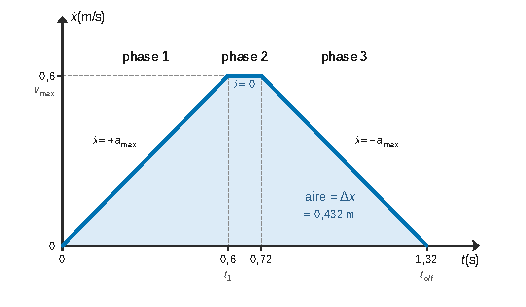
\includegraphics{figures/q05-profil-vitesse-trapeze.pdf}
\caption*{Figure 1 --- Loi de vitesse en trapèze du moule : accélération, palier,
décélération ; l'aire sous la courbe vaut Δx}
\end{figure}

\hypertarget{question-6}{%
\subsection{Question 6}\label{question-6}}

Phases d'accélération et de décélération :

\equationajustee{\begin{aligned}
t_1=t_3&=\frac{v_{max}}{a_{max}}\\
&=0{,}6\ \text{s}\\
d_1=d_3&=\frac{v_{max}^2}{2a_{max}}\\
&=0{,}18\ \text{m}
\end{aligned}}

Comme \(d_1+d_3=0{,}36\ \text{m}<\Delta x\), le palier existe :

\equationajustee{\begin{aligned}
d_2&=\Delta x-d_1-d_3\\
&=0{,}432-0{,}36=0{,}072\ \text{m}\\
t_2&=\frac{d_2}{v_{max}}\\
&=0{,}12\ \text{s}
\end{aligned}}

\equationajustee{\begin{aligned}
t_{o/f}&=t_1+t_2+t_3\\
&=\frac{\Delta x}{v_{max}}+\frac{v_{max}}{a_{max}}\\
&=0{,}72+0{,}60
\end{aligned}}

\equationajustee{\boxed{t_{o/f}=1{,}32\ \text{s}}}

\hypertarget{question-7}{%
\subsection{Question 7}\label{question-7}}

Les quatre étapes se succèdent sans chevauchement (plastification en temps masqué) ; l'ouverture et la fermeture durent chacune \(t_{o/f}\) :

\equationajustee{\boxed{t_{cycl}=t_f+t_i+t_o+t_e=2\,t_{o/f}+t_i+t_e}}

\equationajustee{\begin{aligned}
t_{cycl}&=2\times1{,}32+1{,}39+1{,}0\\
&\simeq5{,}03\ \text{s}
\end{aligned}}

\hypertarget{question-8}{%
\subsection{Question 8}\label{question-8}}

On compare \(t_{cycl}\simeq5{,}03\) s à \(t_{moy}=6{,}0\) s : \(t_{cycl}<t_{moy}\).

La cadence atteignable vaut \(10\times3600/5{,}03\simeq7{,}15\cdot10^3\) pièces/h, supérieure à \(6000\) pièces/h.

\textbf{L'exigence « 112 » est respectée}, avec une marge d'environ \(1\) s par cycle.

\hypertarget{partie-3-uxe9tude-guxe9omuxe9trique-et-cinuxe9matique}{%
\section{Partie 3 --- Étude géométrique et cinématique}\label{partie-3-uxe9tude-guxe9omuxe9trique-et-cinuxe9matique}}

\hypertarget{question-9}{%
\subsection{Question 9}\label{question-9}}

Les trois bases se déduisent de \((\vec x_0,\vec y_0,\vec z_0)\) par des rotations d'axe \(\vec z_0\) (figures planes, \(\vec z_0\) sortant) :

\begin{itemize}
\tightlist
\item
  d'angle \(\beta\) : \(\vec x_2=\cos\beta\,\vec x_0+\sin\beta\,\vec y_0\) et \(\vec y_2=-\sin\beta\,\vec x_0+\cos\beta\,\vec y_0\) ;
\item
  d'angle \(\theta\) : \(\vec x_3=\cos\theta\,\vec x_0+\sin\theta\,\vec y_0\) et \(\vec y_3=-\sin\theta\,\vec x_0+\cos\theta\,\vec y_0\) ;
\item
  d'angle \(\varphi\) : \(\vec x_4=\cos\varphi\,\vec x_0+\sin\varphi\,\vec y_0\) et \(\vec y_4=-\sin\varphi\,\vec x_0+\cos\varphi\,\vec y_0\).
\end{itemize}

\begin{figure}[H]
\centering
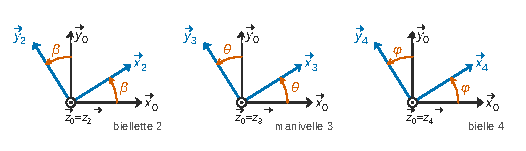
\includegraphics{figures/q09-figures-changement-base.pdf}
\caption*{Figure 2 --- Figures de changement de base : rotations d'axe z0 d'angles
β, θ, φ (dessinés positifs)}
\end{figure}

Les angles sont dessinés positifs ; sur la figure 7 du sujet, \(\beta\) et \(\varphi\) sont négatifs dans la position représentée, ce qui ne change pas les relations de projection.

\hypertarget{question-10}{%
\subsection{Question 10}\label{question-10}}

Fermeture géométrique sur \(OABO\), avec \(\vec{BO}=-\vec{OB}=-e\,\vec x_3\) :

\equationajustee{\vec{OA}+\vec{AB}+\vec{BO}=\vec 0}

\equationajustee{\lambda\,\vec x_0+h\,\vec y_0+d\,\vec x_2-e\,\vec x_3=\vec 0}

En projection sur \(\vec x_0\) et \(\vec y_0\) (deux équations scalaires) :

\equationajustee{\boxed{\begin{cases}\lambda+d\cos\beta-e\cos\theta=0\\ h+d\sin\beta-e\sin\theta=0\end{cases}}}

\hypertarget{question-11}{%
\subsection{Question 11}\label{question-11}}

On isole les termes en \(\beta\) :

\equationajustee{\begin{aligned}
d\cos\beta&=e\cos\theta-\lambda\\
d\sin\beta&=e\sin\theta-h
\end{aligned}}

En élevant au carré et en sommant (\(\cos^2\beta+\sin^2\beta=1\)) :

\equationajustee{\begin{aligned}
d^2&=(e\cos\theta-\lambda)^2+(e\sin\theta-h)^2\\
&=e^2+\lambda^2+h^2-2e\lambda\cos\theta-2eh\sin\theta
\end{aligned}}

d'où \(P\cos\theta+Q\sin\theta=R\) avec

\equationajustee{\boxed{\begin{aligned}
P&=2e\lambda\\
Q&=2eh\\
R&=\lambda^2+h^2+e^2-d^2
\end{aligned}}}

\hypertarget{question-12}{%
\subsection{Question 12}\label{question-12}}

En divisant par \(\sqrt{P^2+Q^2}\) et avec la définition de \(\psi\) :

\equationajustee{\begin{aligned}
\cos\theta\cos\psi+\sin\theta\sin\psi&=\frac{R}{\sqrt{P^2+Q^2}}\\
\cos(\theta-\psi)&=\frac{R}{\sqrt{P^2+Q^2}}
\end{aligned}}

donc

\equationajustee{\theta=\psi\pm\arccos\frac{R}{\sqrt{P^2+Q^2}}}

Détermination de \(\psi\) : comme \(\tan\psi=Q/P\), on a \(\psi=\arctan\dfrac{Q}{P}\) lorsque \(P>0\) (c'est-à-dire \(\lambda>0\)).

Comme \(Q=2eh>0\), on a \(\sin\psi>0\) et \(\psi\in\left]0,\pi\right[\).

Lorsque \(P<0\) (\(\lambda<0\), ce qui arrive pendant l'ouverture), il faut prendre \(\psi=\arctan\dfrac{Q}{P}+\pi\) ; pour \(P=0\), \(\psi=\pi/2\).

Une écriture valable dans tous les cas est \(\psi=\arccos\dfrac{P}{\sqrt{P^2+Q^2}}\).

La branche du mécanisme réel est celle qui donne \(\theta=0\) en position fermée (et \(\theta(0)\simeq20^\circ\) sur la figure 8) :

\equationajustee{\boxed{\theta=\psi-\arccos\frac{R}{\sqrt{P^2+Q^2}}}}

avec \(\psi=\arccos\dfrac{P}{\sqrt{P^2+Q^2}}\). Pour \(\lambda>0\), cela s'écrit aussi :

\equationajustee{\theta=\arctan\frac{Q}{P}-\arccos\frac{R}{\sqrt{P^2+Q^2}}\qquad(\lambda>0)}

L'autre signe correspond à l'autre mode d'assemblage du triangle \(OAB\).

\hypertarget{question-13}{%
\subsection{Question 13}\label{question-13}}

Sur la figure 8 :

\begin{itemize}
\tightlist
\item
  moule fermé, \(\theta=0^\circ\) pour \(\lambda_f\simeq150\) mm ;
\item
  moule ouvert, \(\theta=90^\circ\) pour \(\lambda_o\simeq-210\) mm (en \(\lambda=-150\) mm on ne lit que \(\theta\simeq69^\circ\)).
\end{itemize}

\equationajustee{\begin{aligned}
\Delta\lambda&=\lambda_f-\lambda_o\\
&\simeq150-(-210)=360\ \text{mm}
\end{aligned}}

\equationajustee{\boxed{\Delta\lambda\simeq360\ \text{mm}=0{,}36\ \text{m}}}

\hypertarget{question-14}{%
\subsection{Question 14}\label{question-14}}

\equationajustee{\boxed{\dot\lambda_{moy}=\frac{\Delta\lambda}{\Delta t}}}

\equationajustee{\begin{aligned}
\dot\lambda_{moy}&=\frac{0{,}36}{1{,}2}\\
&=0{,}30\ \text{m/s}
\end{aligned}}

\hypertarget{question-15}{%
\subsection{Question 15}\label{question-15}}

Un tour de vis \(6/0\) fait avancer l'écrou \(1\) (guidé en translation, partie 4) d'un pas \(p_v\). Avec \(N_{6/0}\) en tr/min, la vis fait \(N_{6/0}/60\) tours par seconde :

\equationajustee{\boxed{\dot\lambda_{moy}=\frac{p_v\,N_{6/0}}{60}}\qquad(\dot\lambda\ \text{en m/s},\ p_v\ \text{en m/tr},\ N_{6/0}\ \text{en tr/min})}

\hypertarget{question-16}{%
\subsection{Question 16}\label{question-16}}

Courroie crantée : égalité des vitesses linéaires de la courroie sur les deux poulies, donc \(N_mZ_m=N_{6/0}Z_6\) :

\equationajustee{N_m=N_{6/0}\,\frac{Z_6}{Z_m}}

puis, avec la question 15 :

\equationajustee{\boxed{N_m=\frac{60\,\dot\lambda_{moy}}{p_v}\cdot\frac{Z_6}{Z_m}}}

Application numérique :

\equationajustee{\begin{aligned}
N_{6/0}&=\frac{60\times0{,}30}{0{,}03}\\
&=600\ \text{tr/min}\\
N_m&=600\times\frac{90}{30}
\end{aligned}}

\equationajustee{\boxed{N_m=1800\ \text{tr/min}}}

C'est la vitesse minimale fixée par l'exigence « 1121 ».

\hypertarget{question-17}{%
\subsection{Question 17}\label{question-17}}

Le moule \(5\) étant en translation suivant \(\vec x_0\), \(D\) reste sur l'axe \((O,\vec x_0)\).

Pour \(\theta=90^\circ\), \(\vec{OC}=2e\,\vec y_0\) est orthogonal à \(\vec{OD}\) : le triangle \(OCD\) est rectangle en \(O\), d'hypoténuse \(CD=L\). Théorème de Pythagore :

\equationajustee{\boxed{\|\vec{OD}\|=\sqrt{L^2-4e^2}}}

\equationajustee{\begin{aligned}
\|\vec{OD}\|&=\sqrt{400^2-300^2}\\
&\simeq264{,}6\ \text{mm}
\end{aligned}}

\hypertarget{question-18}{%
\subsection{Question 18}\label{question-18}}

Pour \(\theta=0^\circ\), \(O\), \(C\) et \(D\) sont alignés sur \(\vec x_0\) (position de genouillère, annexe 3) :

\equationajustee{\boxed{\|\vec{OD}\|=2e+L=700\ \text{mm}}}

\begin{figure}[H]
\centering
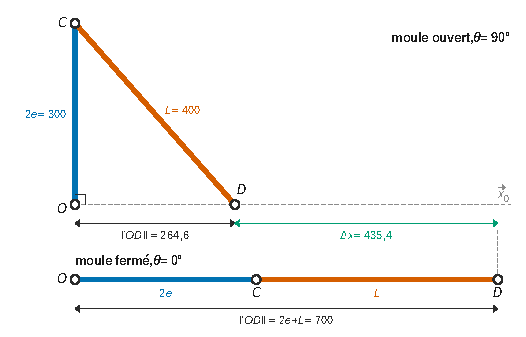
\includegraphics{figures/q17-q18-positions-genouillere.pdf}
\caption*{Figure 3 --- Positions extrêmes de la manivelle 3 et de la bielle 4
(cotes en mm) et course Δx du moule}
\end{figure}

L'amplitude d'ouverture est la différence des deux positions de \(D\) :

\equationajustee{\begin{aligned}
\Delta x&=2e+L-\sqrt{L^2-4e^2}\\
&\simeq700-264{,}6
\end{aligned}}

\equationajustee{\boxed{\Delta x\simeq435{,}4\ \text{mm}}}

\(435{,}4\ \text{mm}\geq400\) mm : \textbf{l'exigence « 1211 » est respectée}.

\hypertarget{partie-4-uxe9tude-des-liaisons}{%
\section{Partie 4 --- Étude des liaisons}\label{partie-4-uxe9tude-des-liaisons}}

\hypertarget{question-19}{%
\subsection{Question 19}\label{question-19}}

Liaisons de la figure 10 :

\begin{itemize}
\tightlist
\item
  \(0\)--\(1\) en \(J\) : pivot glissant d'axe \((J,\vec x_0)\) ;
\item
  \(0\)--\(1\) en \(K\) : pivot glissant d'axe \((K,\vec x_0)\) ;
\item
  \(6\)--\(1\) en \(L\) : hélicoïdale d'axe \((L,\vec x_0)\), de pas \(p_v\) ;
\item
  \(6\)--\(0\) en \(M\) : pivot d'axe \((M,\vec x_0)\).
\end{itemize}

Graphe de structure (figure 4) :

\begin{figure}[H]
\centering
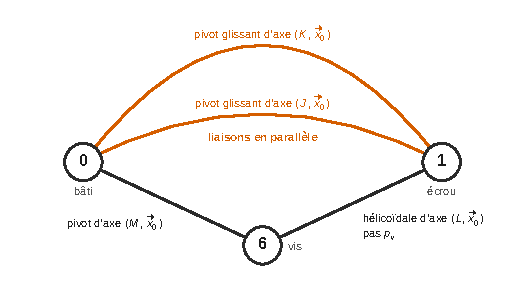
\includegraphics{figures/q19-graphe-structure.pdf}
\caption*{Figure 4 --- Graphe de structure des pièces 0, 1 et 6 : pivots glissants
en J et K en parallèle}
\end{figure}

\textbf{Les liaisons en \(J\) et \(K\) relient le même couple de solides : elles sont en parallèle.}

\hypertarget{question-20}{%
\subsection{Question 20}\label{question-20}}

Pivot glissant d'axe \((K,\vec x_0)\) : rotation et translation suivant \(\vec x_0\) libres, donc résultante et moment nuls suivant \(\vec x_0\).

\equationajustee{\boxed{{}_K\{T_{0\to1}\}=\left\{\begin{matrix}0 & 0\\ Y_K & M_K\\ Z_K & N_K\end{matrix}\right\}_{K,(\vec x_0,\vec y_0,\vec z_0)}}}

\equationajustee{\boxed{{}_K\{V_{1/0}\}=\left\{\begin{matrix}\omega_K & v_K\\ 0 & 0\\ 0 & 0\end{matrix}\right\}_{K,(\vec x_0,\vec y_0,\vec z_0)}}}

\hypertarget{question-21}{%
\subsection{Question 21}\label{question-21}}

Méthode cinématique. Les liaisons étant en parallèle, le torseur cinématique équivalent doit être compatible avec chacune.

En \(J\), de même forme qu'en \(K\) : \(\vec\Omega_{1/0}=\omega_J\vec x_0\) et \(\vec V_{J\in1/0}=v_J\vec x_0\). L'égalité des rotations donne \(\omega_J=\omega_K=\omega\).

On transporte le torseur de \(K\) en \(J\), avec \(\vec{KJ}=\vec{KL}+\vec{LJ}=2a\,\vec z_0\) :

\equationajustee{\begin{aligned}
\vec V_{J\in1/0}&=\vec V_{K\in1/0}+\vec\Omega_{1/0}\wedge\vec{KJ}\\
&=v_K\vec x_0+2a\,\omega\,\vec x_0\wedge\vec z_0\\
&=v_K\vec x_0-2a\,\omega\,\vec y_0
\end{aligned}}

L'identification avec \(v_J\vec x_0\) impose \(\omega=0\) (car \(a\neq0\)) et \(v_J=v_K=v\) :

\equationajustee{\{V_{1/0}\}_{eq}=\left\{\begin{matrix}0 & v\\ 0 & 0\\ 0 & 0\end{matrix}\right\}_{\forall P,(\vec x_0,\vec y_0,\vec z_0)}}

\textbf{La liaison équivalente entre \(0\) et \(1\) est une glissière de direction \(\vec x_0\)} (une mobilité, cinq inconnues statiques transmissibles). L'association est hyperstatique : \(h=8-(6-1)=3\).

\hypertarget{partie-5-dimensionnement-du-moteur}{%
\section{Partie 5 --- Dimensionnement du moteur}\label{partie-5-dimensionnement-du-moteur}}

\hypertarget{question-22}{%
\subsection{Question 22}\label{question-22}}

Cylindre plein de rayon \(d_v/2\) et de longueur \(L_v\), de volume \(\pi\dfrac{d_v^2}{4}L_v\), donc de masse

\equationajustee{m_v=\rho\,\pi\frac{d_v^2}{4}L_v}

\equationajustee{\begin{aligned}
J_v&=\frac{m_v}{2}\left(\frac{d_v}{2}\right)^2\\
&=\frac{m_vd_v^2}{8}\\
&=\frac{\pi\rho L_vd_v^4}{32}
\end{aligned}}

\equationajustee{\boxed{J_v=\frac{m_vd_v^2}{8}=\frac{\pi\rho L_vd_v^4}{32}}}

\hypertarget{question-23}{%
\subsection{Question 23}\label{question-23}}

Maillon par maillon :

\equationajustee{\begin{aligned}
\omega_v&=r\,\omega_m&&\text{(courroie)}\\
\dot\lambda&=\frac{p_v}{2\pi}\,\omega_v&&\text{(vis-\text{écrou}, }p_v\text{ en m/tr, }\omega_v\text{ en rad/s)}\\
\dot x&=i\,\dot\lambda&&\text{(\text{définition} }i=\dot x/\dot\lambda)
\end{aligned}}

D'où

\equationajustee{\boxed{\dot x=\frac{i\,r\,p_v}{2\pi}\,\omega_m}}

Contrôle d'homogénéité : \(p_v/2\pi\) est en m/rad, \(\omega_m\) en rad/s, \(i\) et \(r\) sans dimension, donc \(\dot x\) en m/s. Le facteur \(2\pi\) (nombre de radians par tour) apparaît une seule fois, au dénominateur.

Avec \(k=2{,}4\cdot10^{-3}\) m, \(r=1/3\) et \(p_v=0{,}03\) m/tr, cela correspond à \(i=\dfrac{2\pi k}{r\,p_v}\simeq1{,}5\).

\hypertarget{question-24}{%
\subsection{Question 24}\label{question-24}}

Seuls l'arbre moteur, la vis \(6\) et le moule \(5\) ont une inertie non négligée. L'arbre et la vis tournent autour d'axes fixes, le moule est en translation :

\equationajustee{E_{c(S/0)}=\tfrac12J_m\omega_m^2+\tfrac12J_v\omega_v^2+\tfrac12M\dot x^2}

Avec \(\omega_v=r\,\omega_m\) et \(\dot x=k\,\omega_m\) :

\equationajustee{E_{c(S/0)}=\tfrac12\left(J_m+r^2J_v+Mk^2\right)\omega_m^2}

\equationajustee{\boxed{E_{c(S/0)}=\tfrac12J_{eq}\,\omega_m^2}}

avec

\equationajustee{\boxed{J_{eq}=J_m+r^2J_v+Mk^2}}

\hypertarget{question-25}{%
\subsection{Question 25}\label{question-25}}

Puissances \textbf{extérieures} à \(S\) (actions de l'extérieur de \(S\) sur \(S\)) :

\begin{itemize}
\tightlist
\item
  couple moteur, exercé par le stator (lié au bâti \(0\), extérieur à \(S\)) sur l'arbre moteur : puissance extérieure \(C_m\,\omega_m\) ;
\item
  pesanteur sur le moule \(5\) : le poids \(-Mg\,\vec y_0\) est orthogonal à la vitesse \(\dot x\,\vec x_0\) (translation horizontale), d'où \(-Mg\,\vec y_0\cdot\dot x\,\vec x_0=0\) ;
\item
  pesanteur sur la vis : son centre d'inertie reste sur l'axe fixe, sa vitesse est nulle, puissance nulle ; les autres pièces ont une masse négligée ;
\item
  liaisons avec le bâti (pivots en \(E\)/\(M\) et \(F\), glissière \(0\)/\(1\), guidage du moule, articulations en \(O\)) : parfaites, puissance nulle.
\end{itemize}

Puissances \textbf{intérieures} à \(S\) : liaisons internes (hélicoïdale \(6/1\), pivots en \(A\), \(B\), \(C\), \(D\), transmission poulies-courroie) parfaites, rendements égaux à 1, donc puissance nulle.

\equationajustee{\boxed{P_{ext\to S}=C_m\,\omega_m}}

\equationajustee{\boxed{P_{int}=0}}

\hypertarget{question-26}{%
\subsection{Question 26}\label{question-26}}

Théorème de l'énergie cinétique appliqué à \(S\) dans le repère lié au bâti \(0\), supposé galiléen :

\equationajustee{\frac{\mathrm dE_{c(S/0)}}{\mathrm dt}=P_{ext\to S}+P_{int}}

Avec \(J_{eq}\) constant (\(k\) constant) :

\equationajustee{\begin{aligned}
\frac{\mathrm dE_{c(S/0)}}{\mathrm dt}&=J_{eq}\,\omega_m\dot\omega_m\\
J_{eq}\,\omega_m\dot\omega_m&=C_m\,\omega_m
\end{aligned}}

En simplifiant par \(\omega_m\neq0\) en cours de mouvement :

\equationajustee{\boxed{C_m=J_{eq}\,\dot\omega_m}}

\hypertarget{question-27}{%
\subsection{Question 27}\label{question-27}}

\(\ddot x=k\,\dot\omega_m\), donc

\equationajustee{\begin{aligned}
\dot\omega_m&=\frac{\ddot x}{k}\\
&=\frac{1}{2{,}4\cdot10^{-3}}\\
&\simeq416{,}7\ \text{rad/s}^2
\end{aligned}}

\equationajustee{\begin{aligned}
C_m&=\frac{J_{eq}\,\ddot x}{k}\\
&=2\cdot10^{-2}\times416{,}7
\end{aligned}}

\equationajustee{\boxed{C_m\simeq8{,}3\ \text{N}\cdot\text{m}}}

\hypertarget{question-28}{%
\subsection{Question 28}\label{question-28}}

Il faut \(N_n\geq1900\) tr/min et \(M_n\geq9\) N·m (puissance utile \(9\times1900\times2\pi/60\simeq1{,}79\) kW).

\begin{itemize}
\tightlist
\item
  6 pôles (\(N_n\leq974\) tr/min) et 4 pôles (\(N_n\leq1474\) tr/min) : vitesse insuffisante, exclus.
\item
  2 pôles (\(N_n\simeq2820\) à \(2950\) tr/min) : le LS 90 L (2,2 kW) n'a que \(7{,}30\) N·m ; le premier moteur avec \(M_n\geq9\) N·m est le LS 100 L de 3 kW.
\end{itemize}

\textbf{Moteur retenu : LS 100 L, 2 pôles, \(P_n=3\) kW, \(M_n=10\) N·m, \(N_n=2860\) tr/min} (vitesse nominale compatible avec l'exigence « 1121 »).

\hypertarget{partie-6-vuxe9rification-des-coussinets}{%
\section{Partie 6 --- Vérification des coussinets}\label{partie-6-vuxe9rification-des-coussinets}}

\hypertarget{question-29}{%
\subsection{Question 29}\label{question-29}}

L'effort de fermeture se répartit également entre les 4 bielles :

\equationajustee{\boxed{F_R=\frac{F}{4}}}

\equationajustee{\begin{aligned}
F_R&=\frac{1000\ \text{kN}}{4}\\
&=250\ \text{kN}\\
&=2{,}5\cdot10^5\ \text{N}
\end{aligned}}

\hypertarget{question-30}{%
\subsection{Question 30}\label{question-30}}

Pression rapportée à la surface projetée, rectangle \(d_{int}\times b\) (figure de l'énoncé) :

\equationajustee{\boxed{p=\frac{F_R}{d_{int}\,b}}}

\equationajustee{\begin{aligned}
p&=\frac{2{,}5\cdot10^5}{75\times80}\\
&\simeq41{,}7\ \text{N/mm}^2
\end{aligned}}

\hypertarget{question-31}{%
\subsection{Question 31}\label{question-31}}

La phase étudiée est statique : on compare à \(p_{max}=200\) N/mm². \(p\simeq41{,}7\ \text{N/mm}^2<200\) N/mm² (et même \(<140\) N/mm²).

\textbf{Les coussinets conviennent vis-à-vis de la pression admissible.}

\hypertarget{question-32}{%
\subsection{Question 32}\label{question-32}}

Vitesse de glissement d'un point de l'alésage, de rayon \(d_{int}/2\). La vitesse angulaire est \(\omega_{4/5}=2\pi N_{4/5}/60\) (rad/s, avec \(N_{4/5}\) en tr/min) :

\equationajustee{\begin{aligned}
v_{gliss}&=\omega_{4/5}\,\frac{d_{int}}{2}\\
&=\frac{2\pi N_{4/5}}{60}\cdot\frac{d_{int}}{2}\\
&=\frac{\pi\,d_{int}\,N_{4/5}}{60}
\end{aligned}}

\equationajustee{\boxed{v_{gliss}=\frac{\pi\,d_{int}\,N_{4/5}}{60}}}

\hypertarget{question-33}{%
\subsection{Question 33}\label{question-33}}

Sur la figure 13, \(N_{4/5\,max}\simeq9{,}8\) tr/min (palier entre \(1{,}0\) et \(1{,}2\) s).

\equationajustee{\begin{aligned}
v_{gliss\,max}&=\frac{\pi\times75\times9{,}8}{60}\\
&\simeq38{,}5\ \text{mm/s}
\end{aligned}}

\equationajustee{\boxed{v_{gliss\,max}\simeq38{,}5\ \text{mm/s}<200\ \text{mm/s}}}

\textbf{Les coussinets conviennent aussi vis-à-vis de la vitesse de glissement.}

\hypertarget{partie-7-asservissement-en-tempuxe9rature-du-fourreau}{%
\section{Partie 7 --- Asservissement en température du fourreau}\label{partie-7-asservissement-en-tempuxe9rature-du-fourreau}}

\hypertarget{question-34}{%
\subsection{Question 34}\label{question-34}}

Analogie : potentiel ↔ température, courant ↔ puissance thermique. La source \(P_{th}\) alimente en parallèle \(C_{th}\) et \(R_{th}\), soumis tous deux à \(\Delta\theta=\theta-\theta_a\).

Loi des nœuds (la puissance thermique est un courant) : le courant fourni par la source se partage entre la résistance, qui reçoit \(\Delta\theta/R_{th}\), et le condensateur, qui reçoit \(C_{th}\,\mathrm d\Delta\theta/\mathrm dt\).

\equationajustee{\boxed{P_{th}(t)=\frac{\Delta\theta(t)}{R_{th}}+C_{th}\,\frac{\mathrm d\Delta\theta(t)}{\mathrm dt}}}

(puissance perdue à travers l'isolant + puissance stockée dans l'ensemble fourreau/vis).

\hypertarget{question-35}{%
\subsection{Question 35}\label{question-35}}

Conditions de Heaviside (conditions initiales nulles) : \(\mathcal L\left[\frac{\mathrm d\Delta\theta}{\mathrm dt}\right]=p\,\Delta\theta(p)\).

\equationajustee{\begin{aligned}
P_{th}(p)&=\frac{\Delta\theta(p)}{R_{th}}+C_{th}\,p\,\Delta\theta(p)\\
&=\Delta\theta(p)\left(\frac1{R_{th}}+C_{th}p\right)\\
&=\frac{\Delta\theta(p)}{R_{th}}\left(1+R_{th}C_{th}\,p\right)
\end{aligned}}

(factorisation par \(1/R_{th}\)), d'où

\equationajustee{\boxed{H(p)=\frac{\Delta\theta(p)}{P_{th}(p)}=R_{th}\,\frac{1}{1+R_{th}C_{th}\,p}}}

\hypertarget{question-36}{%
\subsection{Question 36}\label{question-36}}

\textbf{Premier ordre} (dénominateur de degré 1 en \(p\)), \textbf{classe 0} (aucun intégrateur : pas de facteur \(p\) en facteur au dénominateur).

Gain statique \(K=R_{th}=17{,}56\cdot10^{-3}\) K/W, constante de temps \(\tau=R_{th}C_{th}\simeq2775\) s.

\hypertarget{question-37}{%
\subsection{Question 37}\label{question-37}}

Retour unitaire, \(\mathrm{FTBO}(p)=K_pH(p)\) :

\equationajustee{\begin{aligned}
{\mathrm{FTBF}}_1(p)&=\frac{K_pH(p)}{1+K_pH(p)}\\
&=\frac{K_pR_{th}}{1+K_pR_{th}+R_{th}C_{th}\,p}
\end{aligned}}

\equationajustee{\boxed{{\mathrm{FTBF}}_1(p)=\frac{K_{BF}}{1+\tau_{BF}\,p}}}

\equationajustee{\boxed{\begin{aligned}
K_{BF}&=\frac{K_pR_{th}}{1+K_pR_{th}}\\
\tau_{BF}&=\frac{R_{th}C_{th}}{1+K_pR_{th}}
\end{aligned}}}

Premier ordre de classe 0, gain statique inférieur à 1.

\hypertarget{question-38}{%
\subsection{Question 38}\label{question-38}}

La FTBF est du premier ordre, de coefficients tous positifs. Son pôle unique

\equationajustee{p_1=-\frac{1+K_pR_{th}}{R_{th}C_{th}}}

est réel et strictement négatif pour tout \(K_p>0\) : un premier ordre à coefficients positifs est stable quel que soit le gain.

\textbf{Le système bouclé est stable : aucun problème de stabilité.}

\hypertarget{question-39}{%
\subsection{Question 39}\label{question-39}}

D'après le schéma bloc, l'écart est la différence entre la consigne et la sortie, et la sortie vaut \(\theta(p)=K_pH(p)\,\varepsilon(p)\) :

\equationajustee{\begin{aligned}
\varepsilon(p)&=\theta_c(p)-\theta(p)\\
&=\theta_c(p)-K_pH(p)\,\varepsilon(p)
\end{aligned}}

\equationajustee{\boxed{\varepsilon(p)=\frac{\theta_c(p)}{1+K_pH(p)}=\frac{1+R_{th}C_{th}\,p}{1+K_pR_{th}+R_{th}C_{th}\,p}\,\theta_c(p)}}

\hypertarget{question-40}{%
\subsection{Question 40}\label{question-40}}

Théorème de la valeur finale (applicable : système stable, question 38), avec \(\theta_c(p)=\theta_c/p\) :

\equationajustee{\begin{aligned}
\varepsilon_\infty&=\lim_{p\to0}p\,\varepsilon(p)\\
&=\lim_{p\to0}\frac{1+R_{th}C_{th}\,p}{1+K_pR_{th}+R_{th}C_{th}\,p}\,\theta_c\\
&=\frac{\theta_c}{1+K_pR_{th}}
\end{aligned}}

\equationajustee{\boxed{\varepsilon_r=\frac{\varepsilon_\infty}{\theta_c}=\frac1{1+K_pR_{th}}}}

Exigence « 142 » :

\equationajustee{\frac1{1+K_pR_{th}}<10^{-3}\iff K_pR_{th}>999}

\equationajustee{\boxed{K_p>\frac{999}{R_{th}}\simeq5{,}69\cdot10^4\ \text{W/K}}}

\hypertarget{question-41}{%
\subsection{Question 41}\label{question-41}}

\(\varepsilon_r\) et \(\tau_{BF}\) sont tous deux divisés par \(1+K_pR_{th}\) : \textbf{il faut augmenter \(K_p\)}, ce qui améliore à la fois la précision et la rapidité (la limite viendra de la puissance disponible, questions 45 à 48).

\hypertarget{question-42}{%
\subsection{Question 42}\label{question-42}}

Un \textbf{correcteur à action intégrale} (intégral ou proportionnel-intégral) : il rend la boucle ouverte de classe 1, l'erreur statique vis-à-vis d'un échelon est alors nulle quel que soit le gain.

\hypertarget{question-43}{%
\subsection{Question 43}\label{question-43}}

\(K_pR_{th}=60\,000\times17{,}56\cdot10^{-3}=1053{,}6\), d'où

\equationajustee{\begin{aligned}
\tau_{BF}&=\frac{2774{,}5}{1054{,}6}\\
&\simeq2{,}63\ \text{s}\\
t_{r5\%}&=3\,\tau_{BF}
\end{aligned}}

\equationajustee{\boxed{t_{r5\%}\simeq7{,}9\ \text{s}<8\ \text{s}}}

\textbf{L'exigence « 141 » est respectée} (sur le modèle linéaire). En outre \(\varepsilon_r=1/1054{,}6\simeq0{,}095\ \%<0{,}1\ \%\) : l'exigence « 142 » l'est aussi.

\hypertarget{question-44}{%
\subsection{Question 44}\label{question-44}}

\(P_{th}(p)=K_p\,\varepsilon(p)\), donc, avec la question 39 :

\equationajustee{\boxed{P_{th}(p)=\frac{K_p}{1+K_pH(p)}\,\theta_c(p)=\frac{K_p\,(1+R_{th}C_{th}\,p)}{1+K_pR_{th}+R_{th}C_{th}\,p}\,\theta_c(p)}}

\hypertarget{question-45}{%
\subsection{Question 45}\label{question-45}}

Théorème de la valeur initiale avec \(\theta_c(p)=220/p\) :

\equationajustee{\begin{aligned}
P_{th}(0^+)&=\lim_{p\to\infty}p\,P_{th}(p)\\
&=\lim_{p\to\infty}\frac{K_p\,(1+R_{th}C_{th}\,p)}{1+K_pR_{th}+R_{th}C_{th}\,p}\times220\\
&=220\,K_p
\end{aligned}}

\equationajustee{\boxed{P_{th}(0^+)=1{,}32\cdot10^7\ \text{W}=13{,}2\ \text{MW}}}

soit 440 fois la puissance maximale des colliers (30 kW).

\hypertarget{question-46}{%
\subsection{Question 46}\label{question-46}}

La commande sature à \(P_{max}=30\) kW tant que \(K_p\varepsilon>30\) kW, c'est-à-dire \(\varepsilon>0{,}5\) K. Le système évolue alors en boucle ouverte sous puissance constante :

\equationajustee{\Delta\theta(t)=R_{th}P_{max}\left(1-e^{-t/\tau}\right)}

avec \(R_{th}P_{max}=526{,}8\) K et \(\tau=2775\) s. La montée est limitée par \(P_{max}/C_{th}\simeq0{,}19\) K/s.

\textbf{Le temps de réponse à 5 \% est très fortement augmenté} : le système est ralenti, et non accéléré. Il passe à l'ordre de \(-\tau\ln\left(1-\frac{209}{526{,}8}\right)\simeq1{,}4\cdot10^3\) s au lieu de \(7{,}9\) s.

\hypertarget{question-47}{%
\subsection{Question 47}\label{question-47}}

Le bloc sature la commande \(P_{th}\), qui est une puissance thermique (en watts), et non une tension. Limite haute : puissance maximale des colliers ; limite basse : les colliers ne peuvent pas refroidir.

\equationajustee{\boxed{v_1=30\,000\ \text{W}}}

\equationajustee{\boxed{v_2=0\ \text{W}}}

\hypertarget{question-48}{%
\subsection{Question 48}\label{question-48}}

Sur la figure 18, on mesure directement l'instant où la température franchit \(95\ \%\) de la consigne, soit \(209\) °C : vers \(t\simeq1400\) s ; elle atteint 220 °C vers \(1500\) s.

La réponse n'est pas celle d'un premier ordre (montée quasi linéaire, raccord anguleux à 220 °C) : on ne peut pas mesurer une constante de temps puis multiplier par 3.

\equationajustee{\boxed{t_{r5\%}\simeq1400\ \text{s}\simeq23\ \text{min}}}

à comparer aux \(7{,}9\) s de la question 43 (rapport d'environ 180).

Explication : le calcul de la question 43 suppose un modèle linéaire où l'actionneur fournit toute la puissance demandée ; or la commande initiale demandée est \(13{,}2\) MW pour 30 kW disponibles. La commande reste saturée pendant presque toute la montée (jusqu'à \(\varepsilon\simeq0{,}5\) K) ; la dynamique est alors imposée par la puissance installée et la capacité thermique, non par le correcteur. Le calcul en régime saturé donne \(1402\) s pour atteindre 209 °C, en accord avec la simulation.

\(t_{r5\%}\simeq23\ \text{min}<30\) min : \textbf{l'exigence « 111 » (préchauffage en moins de 30 minutes) est respectée.}

\hypertarget{partie-8-alimentation-de-la-machine-dentrauxeenement-de-la-vis-du-fourreau}{%
\section{Partie 8 --- Alimentation de la machine d'entraînement de la vis du fourreau}\label{partie-8-alimentation-de-la-machine-dentrauxeenement-de-la-vis-du-fourreau}}

\hypertarget{question-49}{%
\subsection{Question 49}\label{question-49}}

Document réponse DR1 :

\begin{longtable}[]{@{}
  >{\raggedright\arraybackslash}p{(\columnwidth - 4\tabcolsep) * \real{0.3925}}
  >{\raggedright\arraybackslash}p{(\columnwidth - 4\tabcolsep) * \real{0.1499}}
  >{\raggedright\arraybackslash}p{(\columnwidth - 4\tabcolsep) * \real{0.4277}}@{}}
\toprule\noalign{}
\begin{minipage}[b]{\linewidth}\raggedright
Courbe
\end{minipage} & \begin{minipage}[b]{\linewidth}\raggedright
Tension
\end{minipage} & \begin{minipage}[b]{\linewidth}\raggedright
Justification
\end{minipage} \\
\midrule\noalign{}
\endhead
\bottomrule\noalign{}
\endlastfoot
quasi continue, environ 200 V, faible ondulation & \(u_3\) & sortie du filtre \\
arches positives de 0 à 325 V, période 10 ms & \(u_2\) & sortie du pont de diodes (redressement double alternance) \\
sinusoïde \(\pm325\) V, période 20 ms & \(u_1\) & tension du réseau (230 V efficaces, 50 Hz) \\
\end{longtable}

\hypertarget{question-50}{%
\subsection{Question 50}\label{question-50}}

Entrée alternative, sortie continue : \textbf{convertisseur alternatif-continu, c'est-à-dire un redresseur} (pont de diodes, non commandé, double alternance).

\hypertarget{question-51}{%
\subsection{Question 51}\label{question-51}}

Si \(T_x\) et \(T_x'\) étaient fermés simultanément, ils relieraient directement les deux bornes de la source de tension \(E\) : \textbf{court-circuit de la source de tension}. Une source de tension impose sa tension quel que soit le courant : le courant ne serait limité que par les résistances parasites et détruirait les interrupteurs. Les commandes d'un même bras sont donc complémentaires.

\hypertarget{question-52}{%
\subsection{Question 52}\label{question-52}}

On repère les potentiels par rapport à la borne négative de \(E\). Le potentiel \(V_x\) du point \(x\) vaut \(E\) si \(T_x\) est fermé.

Il vaut \(0\) si \(T_x'\) est fermé. On en déduit :

\equationajustee{\begin{aligned}
u_{12}&=V_1-V_2\\
u_{23}&=V_2-V_3\\
u_{31}&=V_3-V_1
\end{aligned}}

Les graduations de DR2 se lisent de \(\pi/3\) en \(\pi/3\), de \(0\) à \(2\pi\). Le document imprime par erreur « π/2 » pour \(\pi\) et « 10π/3 » pour \(5\pi/3\).

\begin{longtable}[]{@{}
  >{\raggedright\arraybackslash}p{(\columnwidth - 8\tabcolsep) * \real{0.2000}}
  >{\raggedright\arraybackslash}p{(\columnwidth - 8\tabcolsep) * \real{0.2000}}
  >{\raggedright\arraybackslash}p{(\columnwidth - 8\tabcolsep) * \real{0.2000}}
  >{\raggedright\arraybackslash}p{(\columnwidth - 8\tabcolsep) * \real{0.2000}}
  >{\raggedright\arraybackslash}p{(\columnwidth - 8\tabcolsep) * \real{0.2000}}@{}}
\toprule\noalign{}
\begin{minipage}[b]{\linewidth}\raggedright
\(\omega t\)
\end{minipage} & \begin{minipage}[b]{\linewidth}\raggedright
interrupteurs fermés
\end{minipage} & \begin{minipage}[b]{\linewidth}\raggedright
\(u_{12}\)
\end{minipage} & \begin{minipage}[b]{\linewidth}\raggedright
\(u_{23}\)
\end{minipage} & \begin{minipage}[b]{\linewidth}\raggedright
\(u_{31}\)
\end{minipage} \\
\midrule\noalign{}
\endhead
\bottomrule\noalign{}
\endlastfoot
\([0,\frac\pi3]\) & \(T_1,T_2',T_3\) & \(E\) & \(-E\) & \(0\) \\
\([\frac\pi3,\frac{2\pi}3]\) & \(T_1,T_2',T_3'\) & \(E\) & \(0\) & \(-E\) \\
\([\frac{2\pi}3,\pi]\) & \(T_1,T_2,T_3'\) & \(0\) & \(E\) & \(-E\) \\
\([\pi,\frac{4\pi}3]\) & \(T_1',T_2,T_3'\) & \(-E\) & \(E\) & \(0\) \\
\([\frac{4\pi}3,\frac{5\pi}3]\) & \(T_1',T_2,T_3\) & \(-E\) & \(0\) & \(E\) \\
\([\frac{5\pi}3,2\pi]\) & \(T_1',T_2',T_3\) & \(0\) & \(-E\) & \(E\) \\
\end{longtable}

Sur chaque intervalle, \(u_{12}+u_{23}+u_{31}=0\).

\hypertarget{question-53}{%
\subsection{Question 53}\label{question-53}}

On part des définitions lues sur la figure 21 :

\equationajustee{\begin{aligned}
u_{12}&=v_1-v_2\\
u_{23}&=v_2-v_3\\
u_{31}&=v_3-v_1
\end{aligned}}

Alors, avec \(v_2+v_3=-v_1\) :

\equationajustee{\begin{aligned}
u_{12}-u_{31}&=(v_1-v_2)-(v_3-v_1)\\
&=2v_1-(v_2+v_3)\\
&=3v_1
\end{aligned}}

De même :

\equationajustee{\begin{aligned}
u_{23}-u_{12}&=2v_2-(v_1+v_3)\\
&=3v_2\\
u_{31}-u_{23}&=2v_3-(v_1+v_2)\\
&=3v_3
\end{aligned}}

\equationajustee{\boxed{\begin{aligned}
v_1&=\tfrac13(u_{12}-u_{31})\\
v_2&=\tfrac13(u_{23}-u_{12})\\
v_3&=\tfrac13(u_{31}-u_{23})
\end{aligned}}}

\hypertarget{question-54}{%
\subsection{Question 54}\label{question-54}}

\begin{longtable}[]{@{}llll@{}}
\toprule\noalign{}
\(\omega t\) & \(v_1\) & \(v_2\) & \(v_3\) \\
\midrule\noalign{}
\endhead
\bottomrule\noalign{}
\endlastfoot
\([0,\frac\pi3]\) & \(E/3\) & \(-2E/3\) & \(E/3\) \\
\([\frac\pi3,\frac{2\pi}3]\) & \(2E/3\) & \(-E/3\) & \(-E/3\) \\
\([\frac{2\pi}3,\pi]\) & \(E/3\) & \(E/3\) & \(-2E/3\) \\
\([\pi,\frac{4\pi}3]\) & \(-E/3\) & \(2E/3\) & \(-E/3\) \\
\([\frac{4\pi}3,\frac{5\pi}3]\) & \(-2E/3\) & \(E/3\) & \(E/3\) \\
\([\frac{5\pi}3,2\pi]\) & \(-E/3\) & \(-E/3\) & \(2E/3\) \\
\end{longtable}

\begin{figure}[H]
\centering
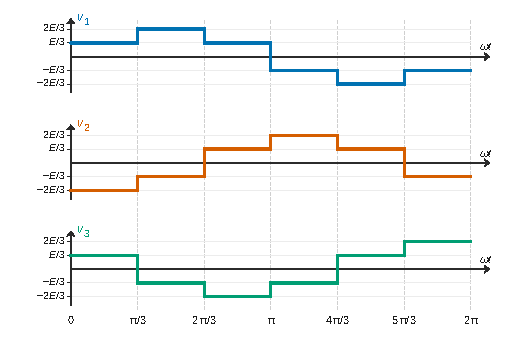
\includegraphics{figures/q54-tensions-simples.pdf}
\caption*{Figure 5 --- Tensions simples v1, v2, v3 de l'onduleur pleine onde sur
une période}
\end{figure}

Avec \(E=200\) V : \(E/3\simeq66{,}7\) V et \(2E/3\simeq133{,}3\) V.

Chaque tension simple est une onde « en marches d'escalier » à six paliers, de période \(2\pi\), symétrique : \(v(\omega t+\pi)=-v(\omega t)\).

Les tensions \(v_2\) et \(v_3\) sont \(v_1\) retardée de \(2\pi/3\) et \(4\pi/3\). La somme des trois est nulle sur chaque intervalle.

\hypertarget{partie-9-protocole-de-communication-module-moteur-et-capteur-du-robot-de-duxe9chargement}{%
\section{Partie 9 --- Protocole de communication module moteur et capteur du robot de déchargement}\label{partie-9-protocole-de-communication-module-moteur-et-capteur-du-robot-de-duxe9chargement}}

\hypertarget{question-55}{%
\subsection{Question 55}\label{question-55}}

Un protocole \textbf{full-duplex} permet d'émettre et de recevoir \textbf{simultanément} dans les deux sens, grâce à deux canaux distincts (TxD broche 3, RxD broche 2, masse commune broche 5).

\hypertarget{question-56}{%
\subsection{Question 56}\label{question-56}}

\textbf{Asynchrone} : aucun signal d'horloge n'est transmis avec les données ; émetteur et récepteur utilisent chacun leur horloge locale. (Le terme n'a rien à voir avec la machine asynchrone ni avec un glissement.)

Le \textbf{bit de start} (passage de l'état de repos 1 à 0) crée un front qui signale le début de trame et resynchronise le récepteur, qui échantillonne ensuite chaque bit au milieu de sa durée.

Il faut donc \textbf{régler au préalable la même vitesse de transmission} (débit en bauds) et le même format de trame (8 bits de données, parité, 2 bits de stop) sur la centrale de gestion et sur chaque module d'axe.

\hypertarget{question-57}{%
\subsection{Question 57}\label{question-57}}

\textbf{Principe} : l'émetteur ajoute un bit choisi pour que le nombre total de bits à 1 (données + parité) soit pair (parité paire) ou impair (parité impaire) ; le récepteur refait le comptage.

\textbf{Utilité} : détecter une erreur de transmission.

\textbf{Limitation} : seul un nombre impair de bits erronés est détecté (deux inversions se compensent) et l'erreur n'est ni localisée ni corrigée.

\hypertarget{question-58}{%
\subsection{Question 58}\label{question-58}}

Chaque trame transporte 8 bits de données ; la position est codée sur 16 bits : \textbf{2 trames}.

\hypertarget{question-59}{%
\subsection{Question 59}\label{question-59}}

\equationajustee{\begin{aligned}
q&=\frac{1500}{2^{16}}\\
&=\frac{1500}{65\,536}\\
&\simeq0{,}023\ \text{mm}
\end{aligned}}

\equationajustee{\boxed{q\simeq0{,}023\ \text{mm}}}

\(0{,}023\ \text{mm}<0{,}05\) mm : \textbf{l'exigence « 152 » est respectée} (du point de vue de la résolution du capteur).

\hypertarget{question-60}{%
\subsection{Question 60}\label{question-60}}

Les curseurs encadrent un bit : \(\Delta=52{,}00\ \mu\)s. Donc \(T_{bit}=52\ \mu\)s et

\equationajustee{\boxed{D=\frac1{T_{bit}}\simeq19\,230\ \text{bit/s}}}

soit le débit normalisé de 19 200 bauds.

\hypertarget{question-61}{%
\subsection{Question 61}\label{question-61}}

Lecture par tranches de \(52\ \mu\)s à partir du front descendant du start (niveau haut = 1). Le bit de start, le bit de parité et les bits de stop ne font pas partie de la donnée :

\begin{longtable}[]{@{}lll@{}}
\toprule\noalign{}
bit & trame 1 & trame 2 \\
\midrule\noalign{}
\endhead
\bottomrule\noalign{}
\endlastfoot
start & 0 & 0 \\
\(b_0\) (poids faible) & 1 & 1 \\
\(b_1\) & 0 & 1 \\
\(b_2\) & 0 & 0 \\
\(b_3\) & 0 & 0 \\
\(b_4\) & 0 & 0 \\
\(b_5\) & 0 & 1 \\
\(b_6\) & 1 & 1 \\
\(b_7\) (poids fort) & 0 & 0 \\
parité & 0 & 0 \\
stop & 1 1 & 1 1 \\
\end{longtable}

Bits de poids faible en premier : l'octet de la trame 1 s'écrit \(0100\,0001_2\) et celui de la trame 2 \(0110\,0011_2\) (parité paire vérifiée dans les deux cas : deux puis quatre bits à 1).

La trame 1 porte l'octet de poids faible, la trame 2 l'octet de poids fort (données émises en commençant par le poids faible). Le nombre de 16 bits est :

\equationajustee{N=0110\,0011\,0100\,0001_2=6341_{16}}

\equationajustee{\boxed{N=25\,409}}

\hypertarget{question-62}{%
\subsection{Question 62}\label{question-62}}

(Le sujet renvoie aux questions 58 et 60 ; il s'agit du quantum de la question 59 et de la valeur de la question 61.)

\equationajustee{\begin{aligned}
x&=N\,q\\
&=25\,409\times\frac{1500}{65\,536}\\
&\simeq581{,}6\ \text{mm}
\end{aligned}}

\equationajustee{\boxed{x\simeq581{,}6\ \text{mm}}}

\hypertarget{question-63}{%
\subsection{Question 63}\label{question-63}}

Une trame compte \(1+8+1+2=12\) bits ; deux trames enchaînées sans temps mort :

\equationajustee{\begin{aligned}
t_{min}&=24\,T_{bit}\\
&=24\times52\ \mu\text{s}\\
&\simeq1{,}25\ \text{ms}
\end{aligned}}

\equationajustee{\boxed{t_{min}\simeq1{,}25\ \text{ms}}}

\hypertarget{question-64}{%
\subsection{Question 64}\label{question-64}}

Seuils, en valeurs numériques codées sur 16 bits (écrites en décimal) :

\equationajustee{\begin{aligned}
\frac{375}{1500}\times65\,536&=16\,384\\
\frac{750}{1500}\times65\,536&=32\,768
\end{aligned}}

\begin{lstlisting}
--- DEBUT ALGORITHME ---
Limite_inf_x0 = 16384
Limite_sup_x0 = 32768
Valeur = lire_capteur_x0
SI (Valeur < Limite_inf_x0) OU (Valeur > Limite_sup_x0)
    Allumer_alarme
--- FIN ALGORITHME ---
\end{lstlisting}

Le mot-clé utile est \textbf{SI} : la valeur n'étant pas relue dans le bloc, un \texttt{TANT\ QUE} bouclerait indéfiniment ; le test est réexécuté à chaque nouvelle lecture du capteur. Pour la position de la question 62 (\(25\,409\)), aucune alarme n'est déclenchée.

\end{document}
